\documentclass[english,greek]{beamer}
\usetheme{Berlin}
\setbeamersize{text margin left=5mm,text margin right=5mm} % set lef right margins
%\usecolortheme{beaver}
%%%%%%%%%%%%%%%%%%%%%%%%% packages %%%%%%%%%%%%%%%%%%%%%%%%%%%%%%%%%%%%
\usepackage{babel} % load greek, english languages
\usepackage[utf8]{inputenc} % Required for inputting international characters
\usepackage[T1]{fontenc} % Output font encoding for international characters
\graphicspath{ {images/} }
\usepackage{graphicx}
\usepackage{subcaption}
\usepackage{comment}
\usepackage{xfrac}
\usepackage{xcolor}
\usepackage[autostyle=true]{csquotes} % Required to generate language-dependent quotes in the bibliography
\MakeOuterQuote{"}
\defineshorthand{;}{?}


\usepackage{ragged2e} % for aligning columns

%%%%%%%%%%%%%%%%%%%%%%%%% shortcuts %%%%%%%%%%%%%%%%%%%%%%%%%%%%%%%%%%%
\def\e{\selectlanguage{english}} % define convenience shortcut for changing language
\def\g{\selectlanguage{greek}} % define convenience shortcut for changing language

%%%%%%%%%%%%%%%%%%%%%%%% information %%%%%%%%%%%%%%%%%%%%%%%%%%%%%%%%%%
\title{Στερεοσκοπική όραση με χρήση νευρωνικού δικτύου}
\author{Βασίλης Γκολέμης}
\institute{Ομάδα κατανόησης πολυμέσων\\
Εργαστήριο Επεξεργασίας Πληροφορίας\\
Αριστοτέλειο Πανεπιστήμιο Θεσσαλονίκης
}
\author[Βασίλης Γκολέμης]{Βασίλης Γκολέμης\\{\footnotesize Επιβλέπων: Αναστάσιος Ντελόπουλος}}

%%%%%%%%%%%%%%%%%%%%%%%% document %%%%%%%%%%%%%%%%%%%%%%%%%%%%%%%%%%%%%
\begin{document}

%%%%%%%%%%%%%%%%%%%%%%%%%%%%% new frame %%%%%%%%%%%%%%%%%%%%%%%%%%%%%%%%%%%%%%%
\begin{frame}
\titlepage
\end{frame}

%%%%%%%%%%%%%%%%%%%%%%%%%%%%% new frame %%%%%%%%%%%%%%%%%%%%%%%%%%%%%%%%%%%%%%%
\begin{frame}{Κατανόηση $3D$ χώρου}
\fontsize{11}{7.2}\selectfont
Γιατί?
\begin{itemize}
	\item Πλοήγηση (ρομποτική, αυτόνομη οδήγηση, ιατρική)
	\item Αλληλεπίδραση (αυτοματοποίηση παραγωγής) 
	\item Καταγραφή (δημιουργία χάρτη από αεροφωτογραφία)
\end{itemize}

Πως?
\begin{itemize}
	\item \e Lidar \g
	\item Όραση \e (monocular, \textcolor{blue}{stereo}, multiview) \g
	\item Δομημένο φως \e (kinect) \g 
\end{itemize}

\end{frame}

%%%%%%%%%%%%%%%%%%%%%%%%%%%%% new frame %%%%%%%%%%%%%%%%%%%%%%%%%%%%%%%%%%%%%%%
\begin{frame}[t]{Στερεοσκοπική Γεωμετρία}
	\fontsize{11}{7.2}\selectfont
	\begin{columns}[onlytextwidth]
		\column{0.5\textwidth}
		\justifying		
		\begin{itemize}
			\item $P=(X,Y,Z)$
			\item $y^{'} = y$ (στερεοσκοπικός περιορισμός)
			\item $x^{'} = f\dfrac{X}{Z}$
			\item $x = f\dfrac{X - b}{Z}$
			\item $Z = \dfrac{fb}{d}$
			\item $d = x^{'}-x$ (παράλλαξη)
		\end{itemize}
		\vspace{3mm}
		
		Στόχος:
		\begin{itemize}
			\item $ \forall p \in I_L $ βρες $ d $
		\end{itemize}
		\column{0.5\textwidth}
		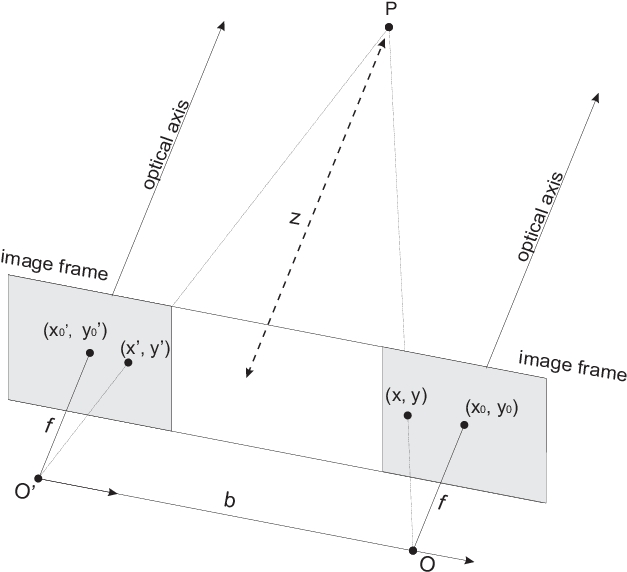
\includegraphics[width=\textwidth]{stereo_geometry.jpg}
	\end{columns}
\end{frame}

%%%%%%%%%%%%%%%%%%%%%%%%%%%%% new frame %%%%%%%%%%%%%%%%%%%%%%%%%%%%%%%%%%%%%%%
\begin{frame}[t]{Χάρτης παράλλαξης}
	\begin{figure}
		\centering
		\begin{subfigure}{0.49\textwidth}
		\includegraphics[width=\textwidth, height = 0.45\textwidth]{motorcycle_l.png}
		\end{subfigure}
		\begin{subfigure}{0.49\textwidth}
		\includegraphics[width=\textwidth, height = 0.45\textwidth]{motorcycle_r.png}
		\end{subfigure}
	\end{figure}
\begin{figure}
	\centering
	\begin{subfigure}{0.49\textwidth}
		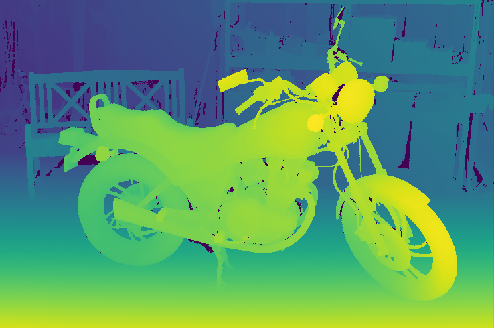
\includegraphics[width=\textwidth, height = 0.45\textwidth]{motorcycle_disp_map_visualization.png}
		\caption{$\mathbf{D}_{\mathbf{ground\_truth}}^L$}
		\label{fig:motorcycle_disp_map} 
	\end{subfigure}
	\begin{subfigure}{0.49\textwidth}
		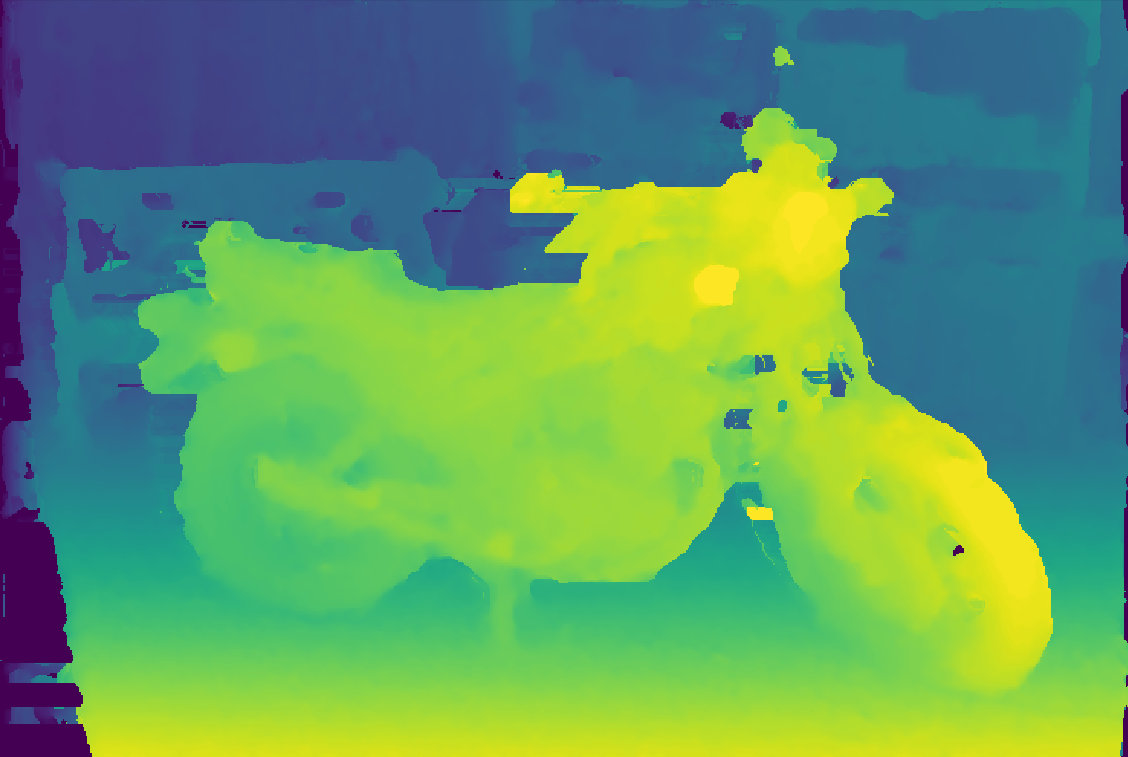
\includegraphics[width=\textwidth, height = 0.45\textwidth]{motorcycle_prediction.png}
		\caption{$\mathbf{D}_{\mathbf{predicted}}^L$}
		\label{fig:motorcycle_pred_disp_map}
	\end{subfigure}
\end{figure}
\end{frame}

%%%%%%%%%%%%%%%%%%%%%%%%%%%%% new frame %%%%%%%%%%%%%%%%%%%%%%%%%%%%%%%%%%%%%%%
\begin{frame}[t]{Αξιολόγηση χάρτη παράλλαξης}
\fontsize{10}{7.2}\selectfont
\begin{itemize}
	\item Απόλυτο σφάλμα πρόβλεψης $\rightarrow$ μέση τιμή ($2.058 px$)
	\item Απόλυτο σφάλμα πρόβλεψης με ανώφλι $\rightarrow$ σφάλμα ($9.891 \%$)
	\item Οπτικοποίηση είτε ως \textcolor{blue}{εικόνα} είτε ως ιστόγραμμα
\end{itemize}
\begin{figure}
	\begin{subfigure}{0.49\textwidth}
		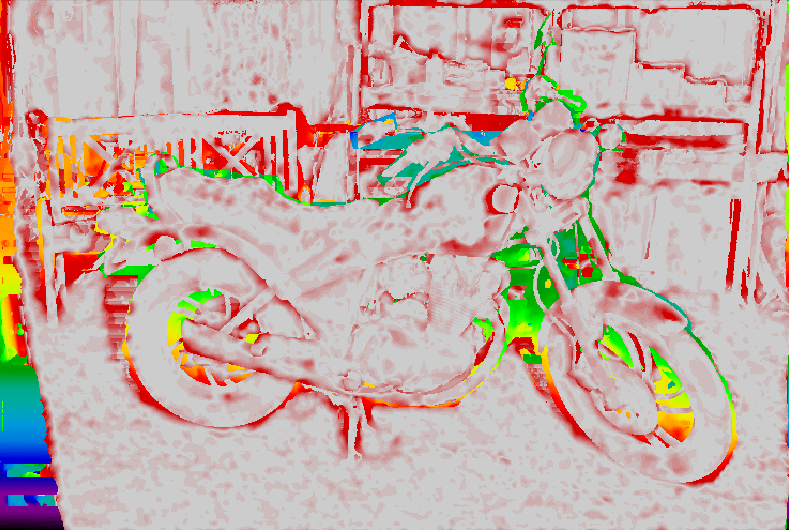
\includegraphics[width=\textwidth, height=30mm]{motorcycle_dist_error.png}
		
		
\includegraphics[width=\textwidth, height=1mm]{error_colorbar.png}
		\caption{\fontsize{7}{7}\selectfont $\mathbf{AD} = |\mathbf{D}_{\mathbf{ground\_truth}}^L - \mathbf{D}_{\mathbf{predicted}}^L| \in [0,60]px$}
	\end{subfigure}
	\begin{subfigure}{0.49\textwidth}
		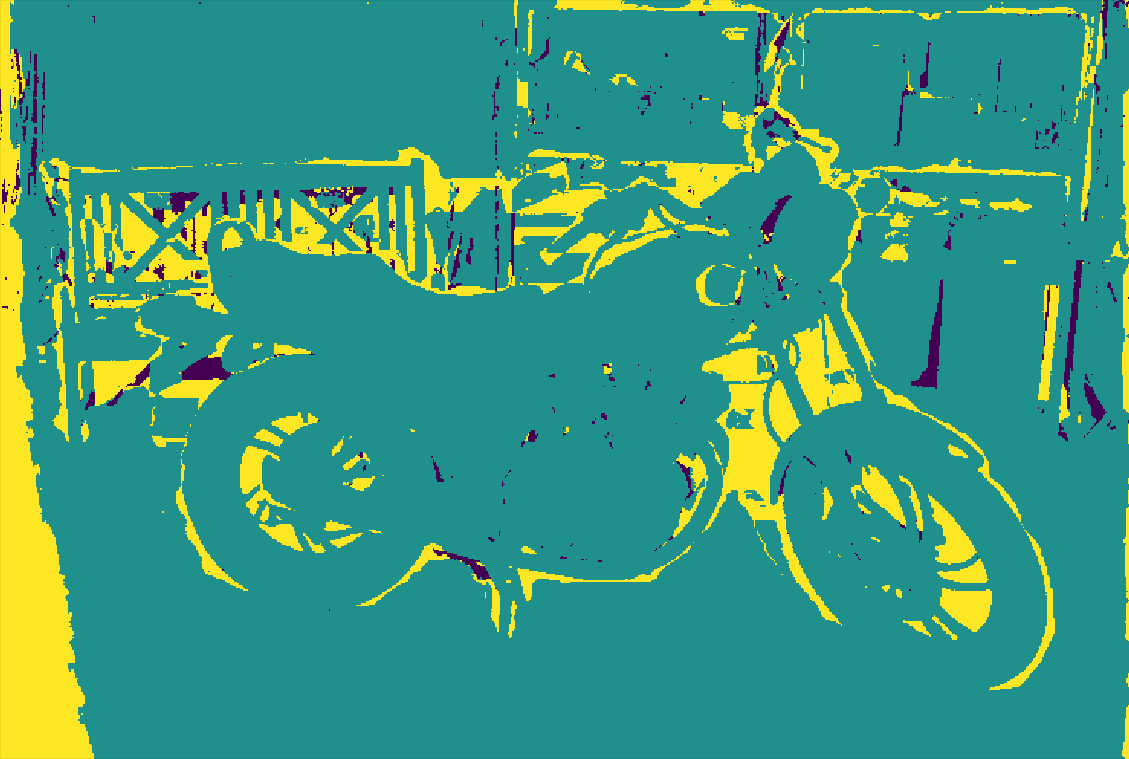
\includegraphics[width=\textwidth, height=31mm]{motorcycle_error.png}
		\caption{\fontsize{6.5}{7} $\mathbf{AD_{threshold}} = |\mathbf{D}_{\mathbf{ground\_truth}}^L - \mathbf{D}_{\mathbf{predicted}}^L| \gtrless 3px$}
	\end{subfigure}

\end{figure}
\end{frame}

%%%%%%%%%%%%%%%%%%%%%%%%%%%%% new frame %%%%%%%%%%%%%%%%%%%%%%%%%%%%%%%%%%%%%%%
\begin{frame}[t]{Πως ψάχνουμε αντίστοιχα σημεία?}
\fontsize{10}{7.2}\selectfont
	\begin{columns}[onlytextwidth]
	\column{0.5\textwidth}
	\e(i) \g \textbf{Ομοιότητα γειτονιάς}:
	\begin{itemize}
		\item Παρόμοιο σχήμα, υφή στις δύο προβολές
		\item \e small baseline (20cm) \g
	\end{itemize}
	\vspace{5mm}
	\e(ii) \g \textbf{Στερεοσκοπικοί περιορισμοί}:
	\begin{itemize}
		\item Περιορισμός συνέχειας/ασυνέχειας
		\item Περιορισμός μοναδικότητας
		\item Συνέπεια διάταξης σημείων			
	\end{itemize}
	\vspace{5mm}
	Ασυνεχείς επιφάνειες $\rightarrow$ ασυνέχειες παράλλαξης + αποκρύψεις $\rightarrow$ πηγή προβλημάτων!
	\column{0.5\textwidth}
	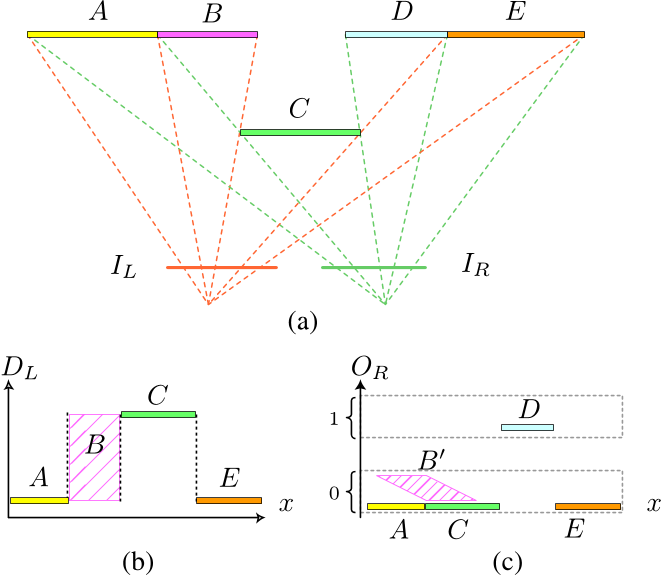
\includegraphics[width=\textwidth]{occlusion_image.png}
	\end{columns}
\end{frame}

%%%%%%%%%%%%%%%%%%%%%%%%%%%%% new frame %%%%%%%%%%%%%%%%%%%%%%%%%%%%%%%%%%%%%%%
\begin{frame}{Περιορισμός μοναδικότητας}
	\begin{columns}[onlytextwidth]
		\column{0.5\textwidth}
		\begin{itemize}
			\item Υπάρχει '1-1' σχέση μεταξύ σημείων αριστερής/δεξιάς λήψης.
			\item Αίρεται όταν υπάρχουν αποκρύψεις
		\end{itemize}	

		\column{0.5\textwidth}
		\begin{figure}
			\centering
			\begin{subfigure}{\textwidth}
			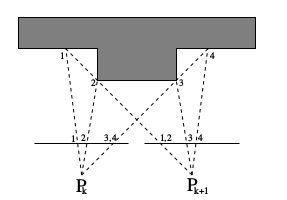
\includegraphics[width=\textwidth, height = 0.5\textwidth]{uniqueness2.png}
			\end{subfigure}
			
			\begin{subfigure}{\textwidth}
			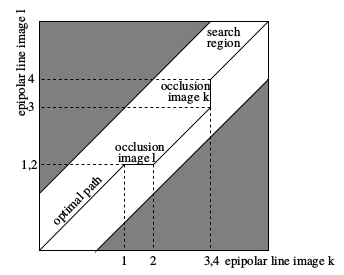
\includegraphics[width=\textwidth, height = 0.5\textwidth]{uniqueness1.png}
			\end{subfigure}
		\end{figure}
	\end{columns}
\end{frame}

%%%%%%%%%%%%%%%%%%%%%%%%%%%%% new frame %%%%%%%%%%%%%%%%%%%%%%%%%%%%%%%%%%%%%%%
\begin{frame}{Συνέπεια διάταξης σημείων}
	\begin{columns}[onlytextwidth]
		\column{0.5\textwidth}		
		\begin{itemize}
			\item Αν για σημεία $p_1,p_2$ της μιας λήψης ισχύει $x_1<x_2$ το ίδιο θα ισχύει και για τα "αντίστοιχα" σημεία τους 
			\item Αίρεται όταν υπάρχουν αποκρύψεις
		\end{itemize}
		\column{0.5\textwidth}
		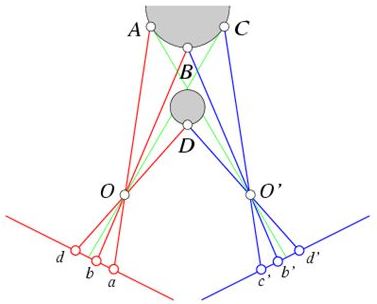
\includegraphics[width=\textwidth]{ordering_constraint_failure.png}
	\end{columns}
\end{frame}

%%%%%%%%%%%%%%%%%%%%%%%%%%%%% new frame %%%%%%%%%%%%%%%%%%%%%%%%%%%%%%%%%%%%%%%
\begin{frame}{Επίλυση Προβλήματος}
Χωρίζουμε το πρόβλημα σε 3 στάδια:
\begin{enumerate}
	\item Δημιουργία πίνακα κόστους: $I^L,I^R\rightarrow C$
	
	$C(d,x,y)$: πόση ομοιότητα εμφανίζει η γειτονιά του $I^L(x,y)$ με αυτή του $I^R(x-d,y)$
	\item $C_{init} \rightarrow C_{optimized} \xrightarrow{argmin_d C(d,x,y)} D_{init}$
	\item $D_{init} \rightarrow D_{optimized}$
\end{enumerate}
\end{frame}

%%%%%%%%%%%%%%%%%%%%%%%%%%%%% new frame %%%%%%%%%%%%%%%%%%%%%%%%%%%%%%%%%%%%%%%
\begin{frame}{Πίνακας $C$: Απλές μέθοδοι \e vs \g Νευρωνικό Δίκτυο}
\fontsize{8}{7.2}\selectfont
	\begin{columns}[onlytextwidth]
		\column{0.5\textwidth}		
		- Άθροισμα απόλυτων διαφορών:
		$$ C(d,p) = -\sum_{q \in N_p} |I^L(q) - I^R(q-d)| $$
		- Ομοιότητα συνημιτόνου:
		\begin{equation*}
			C(\mathbf{p}, d) = \frac{\sum_{\mathbf{q} \in \mathcal{N}_{\mathbf{p}}} I^L(\mathbf{q}) I^R(\mathbf{q} - \mathbf{d})}
			{\sqrt{\sum_{\mathbf{q} \in \mathcal{N}_{\mathbf{p}}} I^L(\mathbf{q})^2 \sum_{\mathbf{q} \in \mathcal{N}_{\mathbf{p}}} I^R(\mathbf{q} - \mathbf{d})^2 }}
		\end{equation*}
		- Απόσταση \e Hamming \g σε μετασχηματισμό \e Census \g
		
		\column{0.5\textwidth}
		
		\textbf{Νευρωνικό Δίκτυο}
		\vspace{3mm}
		
		- Πλεονέκτημα:
		\begin{itemize}
			\item Εξαγωγή βέλτιστου τοπικού περιγραφέα γειτονιάς από τα δεδομένα - ο σχεδιασμός του από προγραμματιστή θα ήταν αδύνατος
			\item Βέλτιστος? Ενσωματώνει ποιοτικά χαρακτηριστικά (σχήμα, υφή κλπ) της γειτονιάς που μένουν αμετάβλητα στις δύο προβολές
		\end{itemize}
		\vspace{2mm}
		- Μειονέκτημα:
		\begin{itemize}
			\item Υπολογιστική πολυπλοκότητα: συνελικτικό νευρωνικό δίκτυο 8 κρυφών επιπέδων. Απαραίτητη η χρήση \e GPU. \g Ακόμα κι έτσι, 
			
			Χρόνος εκτέλεσης $\approx 1 \dfrac{sec}{\text{εικόνα}}$
		\end{itemize}
	\end{columns}
\end{frame}

%%%%%%%%%%%%%%%%%%%%%%%%%%%%% new frame %%%%%%%%%%%%%%%%%%%%%%%%%%%%%%%%%%%%%%%
\begin{frame}{Αρχιτεκτονική νευρωνικού δικτύου}
\fontsize{9}{7.2}\selectfont
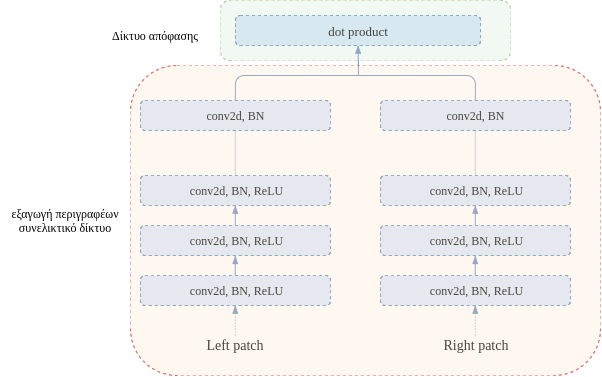
\includegraphics[width=0.8\textwidth]{neural_net_arch.png}
\end{frame}

%%%%%%%%%%%%%%%%%%%%%%%%%%%%% new frame %%%%%%%%%%%%%%%%%%%%%%%%%%%%%%%%%%%%%%%
\begin{frame}{Είσοδοι συνελικτικού νευρωνικού δικτύου}
\fontsize{9}{7.2}\selectfont
Κατά την \textbf{εκπαίδευση}:
\begin{itemize}
	\item \e \textbf{left patch:} \g γειτονιά $N_p$ μεγέθους $[19 \times 19]$ γύρω από σημείο $I^L(\mathbf{p})$
	\item \e \textbf{right patch:} \g χωρίο μεγέθους \e $[(19+\texttt{max\_disparity}) \times 19]$ \g. Το χωρίο περιλαμβάνει τις γειτονιές $N_p$ όλων την υποψήφιων "αντίστοιχων" σημείων $I^R(\mathbf{p-d})$
	\item συνέλιξη χωρίς \e zero-padding \g $\rightarrow$ χωρικές διαστάσεις μειώνονται κατά $2$ σε κάθε μπλοκ ($19-(8\cdot 2) = 1$)
\end{itemize}
\e
\begin{figure}
	\centering
	\begin{subfigure}{0.24\textwidth}
	\centering
	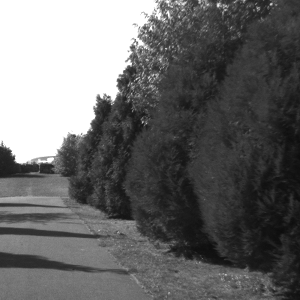
\includegraphics[scale=0.20]{kitti2012_im9_lcrop.png}
	\caption{\e left patch}
	\end{subfigure}
	\begin{subfigure}{0.74\textwidth}
	\centering
	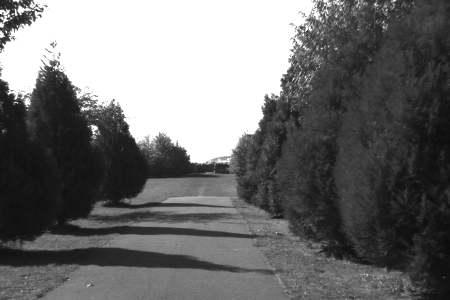
\includegraphics[scale=0.20]{kitti2012_im9_rcrop.png}
	\caption{\e right patch}
	\end{subfigure}
\end{figure}
\g
Κατά την \textbf{εκτέλεση}:
\begin{itemize}
	\item Ολόκληρες εικόνες $I^L, I^R \rightarrow$ με \e zero padding. \g
\end{itemize}

\end{frame}

%%%%%%%%%%%%%%%%%%%%%%%%%%%%% new frame %%%%%%%%%%%%%%%%%%%%%%%%%%%%%%%%%%%%%%%
\begin{frame}{Έξοδοι συνελικτικού νευρωνικού δικτύου}

Κατά την \textbf{εκπαίδευση}:
\begin{itemize}
		\item $I_{desc}^L(\mathbf{p})$: τον \e descriptor \g του \e left patch \g
		\item τους \e $\texttt{max\_disparity}+1$  descriptors \g των αντίστοιχων γειτονιών των σημείων \e $I^R(\mathbf{p-d}) \: \forall d \in [0,\ldots,\texttt{max\_disparity}] $ \g
		\item $I_{desc}^L(\mathbf{p}) \in \mathbb{R}^{64}$
\end{itemize}

Κατά την \textbf{εκτέλεση}:
\begin{itemize}
	\item $I^L_{desc}, I^R_{desc}$: \e descriptors \g κάθε θέσης αριστερής και δεξιάς εικόνες
\end{itemize}
\vspace{4mm}
Το δίκτυο απόφασης λειτουργεί όμοια σε εκπαίδευση/εκτέλεση:
\begin{itemize}
	\item Συγκρίνουμε \e descriptors \g με \e dot product \g
\end{itemize}


\end{frame}



%%%%%%%%%%%%%%%%%%%%%%%%%%%%% new frame %%%%%%%%%%%%%%%%%%%%%%%%%%%%%%%%%%%%%%%
\begin{frame}{Εκπαίδευση}

\begin{itemize}
\fontsize{9}{7.2}\selectfont
	\item Σύγκριση $I_{desc}^L(\mathbf{p})$ και \e $I_{desc}^R(\mathbf{p-d}) \: \forall d \in [0,\ldots,\texttt{max\_disparity}]$. \g Αποθηκεύουμε τις τιμές στο διάνυσμα $similarity$.
	\item $C_{data}$: \e softmax cross entropy \g μεταξύ των διανυσμάτων \e $similarity$ \g και \e $label$ \g (δείχνει την σωστή τιμή παράλλαξης)
	\item $C_{reg} = \lambda \sum_i \Theta_i^2$, προσθέτουμε \e dropout(0.4) \g μετά από κάθε \e ReLU \g 
	\item \e Optimizer: ADAM \g
	\item Εκπαίδευση σε $\approx 4 \times 10^6$ παραδείγματα
	\item \e batch size = 128 \g
\end{itemize}
\centering
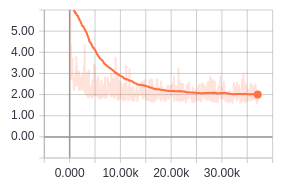
\includegraphics[scale=0.5]{xentropy_mean_loss_over_batch.png}

\end{frame}

%%%%%%%%%%%%%%%%%%%%%%%%%%%%% new frame %%%%%%%%%%%%%%%%%%%%%%%%%%%%%%%%%%%%%%%
\begin{frame}{Εκπαίδευση \e vs \g εκτέλεση}

Γιατί διαφορετικές είσοδοι σε εκπαίδευση και εκτέλεση?
\begin{itemize}
	\item Τρικ για την αύξηση του \e dataset. \g Κάθε εικόνα δημιουργεί $\approx 10^5$ παραδείγματα
	\item \e training set: \g 125 εικόνες $\rightarrow 15 \times 10^6$ 
	\item Τι χάνουμε? Περιορισμός στα \e layers \g που μπορούμε να χρησιμοποιήσουμε. Αποκλείονται \e layers \g που αλλοιώνουν χωρικές διαστάσεις (πχ \e max pool) \g
\end{itemize}

\end{frame}

%%%%%%%%%%%%%%%%%%%%%%%%%%%%% new frame %%%%%%%%%%%%%%%%%%%%%%%%%%%%%%%%%%%%%%%
\begin{frame}{Αποτέλεσμα νευρωνικού δικτύου}
\begin{columns}[onlytextwidth]
\column{0.2\textwidth}
\begin{itemize}
	\item μέσο απόλυτο σφάλμα: $1.132 px$
	\item ποσοστό σφάλματος: $5.846\%$
	\item μέθοδος \e AD-Census: \g $19.84\%$
\end{itemize}
\column{0.8\textwidth}
\begin{figure}
	\centering
	\begin{subfigure}{\textwidth}
	\centering
	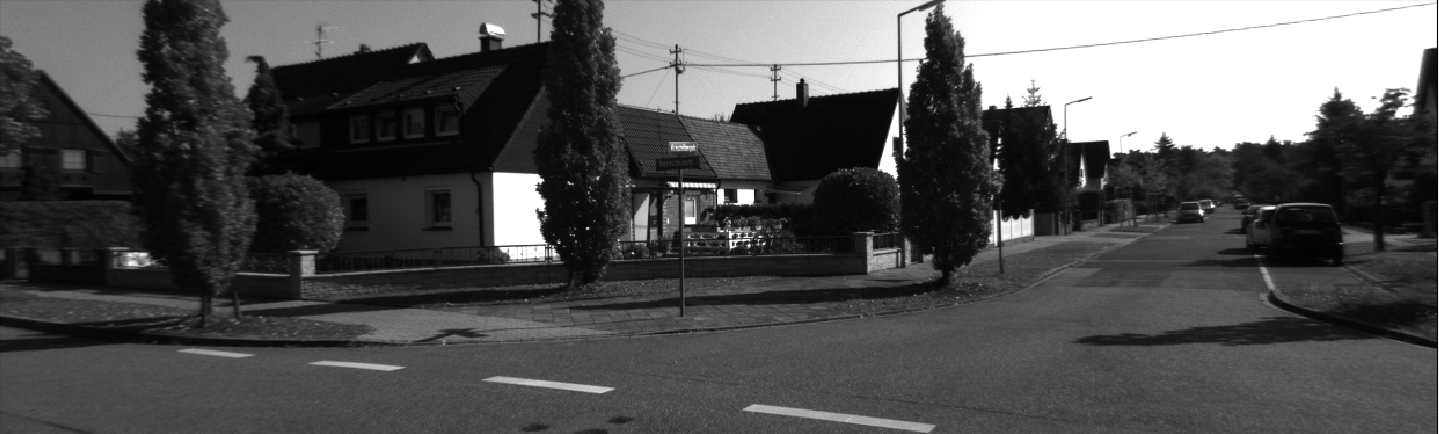
\includegraphics[height=20mm]{im4_imL.png}
	\end{subfigure}
	
	\begin{subfigure}{\textwidth}
	\centering
	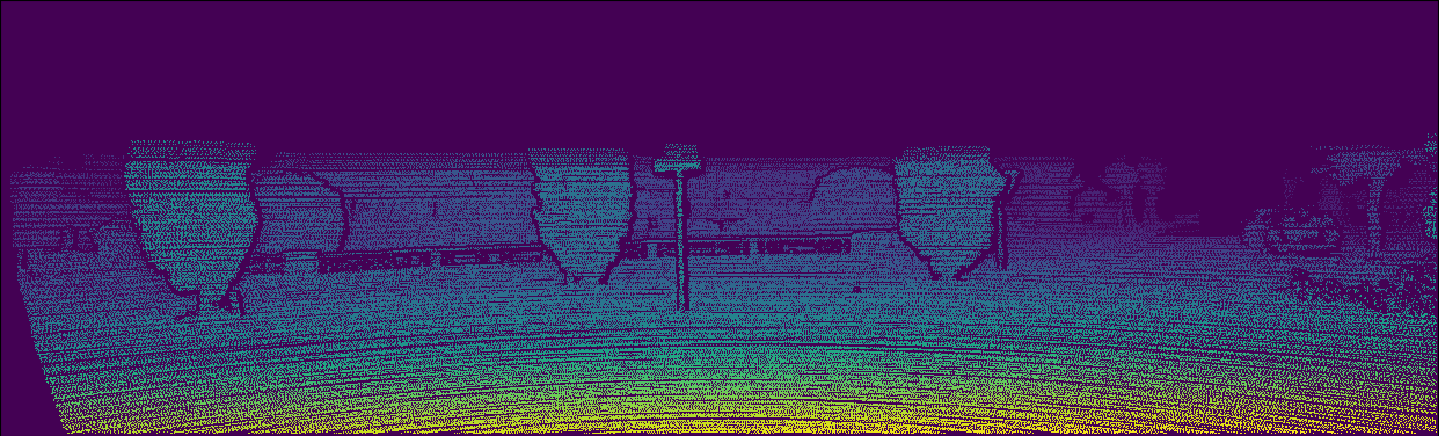
\includegraphics[height=20mm]{im4_disp_gt.png}
	\end{subfigure}
	
	\begin{subfigure}{\textwidth}
	\centering
	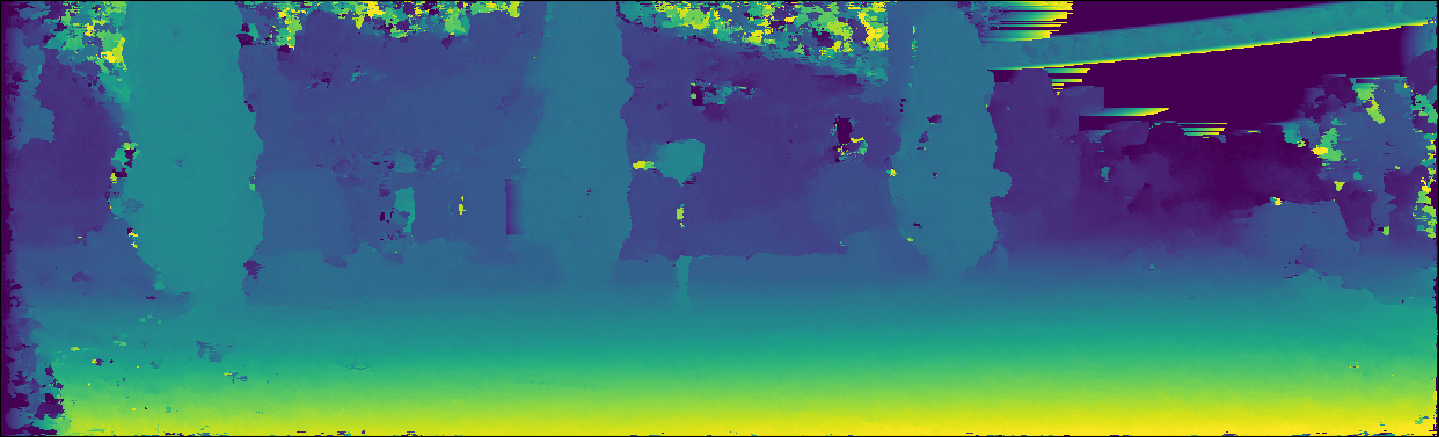
\includegraphics[height=20mm]{im4_luo_cnn_disp.png}
	\end{subfigure}
\end{figure}
\end{columns}

\end{frame}

%%%%%%%%%%%%%%%%%%%%%%%%%%%%% new frame %%%%%%%%%%%%%%%%%%%%%%%%%%%%%%%%%%%%%%%
\begin{frame}{Βήμα 2: $C_{init} \rightarrow C_{optimized}$}
\fontsize{9}{7.2}\selectfont
	\begin{columns}[onlytextwidth]
		\column{0.5\textwidth}
		\begin{itemize}
			\item συνεχείς περιοχές $\rightarrow$ συνεχής παράλλαξη
			\item Προσεκτική δημιουργία γειτονιών $N_p$ με μέθοδο σταυρού \e (Mei et. al 2011)
		\end{itemize}
		\vspace{4mm}
		\g Πήγαινε κάτω, πάνω, αριστερά, δεξιά όσο:
		\vspace{2mm}
		
		\e $|I(\mathbf{p}) - I(\mathbf{p'})| < \texttt{intensity\_threshold}$
		\vspace{2mm}
		
		\e $\|\mathbf{p} - \mathbf{p'}\| < \texttt{distance\_threshold}$
		\g
		\vspace{2mm}
		
		$N_p:$ οριζόντιες ευθείες των σημείων της κάθετης ευθείας του σημείου $p$

		\column{0.5\textwidth}
		\begin{figure}
			\centering
			\begin{subfigure}{\textwidth}
			\centering
			
\includegraphics[height =25mm]{cbca_tsukuba.png}
			\end{subfigure}
			
			\begin{subfigure}{\textwidth}
			\centering
			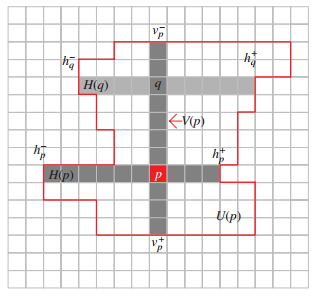
\includegraphics[height =30mm]{cbca_cross.png}
			\end{subfigure}
		\end{figure}
	\end{columns}
\end{frame}

%%%%%%%%%%%%%%%%%%%%%%%%%%%%% new frame %%%%%%%%%%%%%%%%%%%%%%%%%%%%%%%%%%%%%%%
\begin{frame}{Μέσος όρος κόστους σε γειτονιές}
\fontsize{9}{7.2}\selectfont
$\forall C(d,x,y)$:
\begin{itemize}
\item υπολόγισε την τομή των γειτονιών του $Ι^L(x,y)$ και του $Ι^R(x-d,y)$
\item αποθήκευσε ως $C_{opt}(d,x,y)$ το μέσο όρο των $C$ στην παραπάνω γειτονιά
\end{itemize}
\vspace{3mm}

Παρατηρήσεις:
\begin{itemize}
\item υποθέτει: δύο \e pixels \g στην ίδια γειτονιά θα έχουν συνήθως ίδιο ή κοντινό $d$
\item εξομαλύνει αστάθειες στον αρχικό πίνακα κόστους
\item μπορούμε να εφαρμόσουμε το βήμα επαναληπτικά $n$ φορές  
\end{itemize}
\end{frame}

%%%%%%%%%%%%%%%%%%%%%%%%%%%%% new frame %%%%%%%%%%%%%%%%%%%%%%%%%%%%%%%%%%%%%%%
\begin{frame}{\e Semi-global matching (1)}
\fontsize{9}{7.2}\selectfont
\g
\begin{multline*}
E_C(D) = \sum_{\mathbf{p}} \biggl( C(\mathbf{p}, D(\mathbf{p}))
+ \sum_{\mathbf{q} \in \mathcal{N}_{\mathbf{p}}} P_1 \cdot 1\{|D(\mathbf{p}) - D(\mathbf{q})| = 1\} \\
+ \sum_{\mathbf{q} \in \mathcal{N}_{\mathbf{p}}} P_2 \cdot 1\{|D(\mathbf{p}) - D(\mathbf{q})| > 1\} \biggr)
\end{multline*}

Παρατηρήσεις:
\begin{itemize}
\item \e Heiko Hirschmüller - 2008 \g
\item εξομαλύνει τον πίνακα κόστους $C$ λαμβάνοντας υπ' όψη το σύνολο των τιμών του
\item οι "τιμωρίες" $P_1$ και $P_2$ μειώνονται αν οι φωτεινότητες γειτονικών \e pixel \g έχουν μεγάλη απόκλιση (πιθανή ακμή)
\item αδύνατο να επιλυθεί καθολικά, οι πιθανές τιμές του $D$ είναι $(m \times n)^{max\_disparity}$
\item το αντιμετωπίζουμε με δυναμικό προγραμματισμό σε με μεμονωμένες κατευθύνσεις
\end{itemize}
\end{frame}

%%%%%%%%%%%%%%%%%%%%%%%%%%%%% new frame %%%%%%%%%%%%%%%%%%%%%%%%%%%%%%%%%%%%%%%
\begin{frame}{\e Semi-global matching (2)}
\fontsize{9}{7.2}\selectfont
\g
Επιλέγω κατεύθυνση $r$ κι εφαρμόζω αναδρομική σχέση:
\begin{multline*} \label{sgm_recursive} C_{\mathbf{r}}(\mathbf{p}, d) = C(\mathbf{p},
d) - \min_k C_r(\mathbf{p} - \mathbf{r}, k) + \min\biggl\{ C_r(\mathbf{p} -
\mathbf{r}, d), C_r(\mathbf{p} - \mathbf{r}, d - 1) + P_1,\\ C_r(\mathbf{p} -
\mathbf{r}, d + 1) + P_1, \min_k C_{\mathbf{r}}(\mathbf{p} - \mathbf{r}, k) +
P_2 \biggr\}  \end{multline*}

\begin{itemize}
\item Υπολογιστική πολυπλοκότητα $O(directions \cdot max\_disparity \cdot W \cdot H)$
\item όσες περισσότερες κατευθύνσεις τόσο καλύτερο αποτέλεσμα, ο \e Hirschmüller \g προτείνει 16
\item το εφαρμόζουμε σε 4 (πάνω, κάτω, αριστερά, δεξιά) για να γλιτώσουμε πολυπλοκότητα
\end{itemize}
\end{frame}

%%%%%%%%%%%%%%%%%%%%%%%%%%%%% new frame %%%%%%%%%%%%%%%%%%%%%%%%%%%%%%%%%%%%%%%
\begin{frame}{Βήμα 3: $D_{init} \rightarrow D_{opt}$}
\fontsize{9}{7.2}\selectfont
\g
Μετά τις βελτιώσεις στο πεδίο του $C$ υπολογίζουμε τον χάρτη (εικόνα) παράλλαξης με μέθοδο \e winner takes it all: \g

$$D = argmin_d C(d,x,y)$$ 

Υπολογίζουμε χάρτες $D_L, D_R$ θεωρώντας εικόνα αναφοράς $I_L, I_R$ αντίστοιχα και βασιζόμαστε στον περιορισμό μοναδικότητας:

\begin{itemize}
\item \e $|D^L(\textbf{p}) - D^R(\textbf{p}-\textbf{d})| \leqslant 1$ \g, τότε ορθή παράλλαξη και τέλος η αναζήτηση
\item \e $|d - D^R(\textbf{p}-\textbf{d})| > 1 \quad \forall d:\lbrace \textbf{p}-\textbf{d} \geqslant 0 \rbrace$ \g, διατρέχω την επιπολική ευθεία κι ελέγχω ότι κανένα άλλο \e pixel \g δεν αντιστοιχίζεται με το \e pixel $\textbf{p}$ \g $\Rightarrow$ απόκρυψη
\item αν αντίθετα υπάρχει $\Rightarrow$ αστοχία πρόβλεψης
\end{itemize}

Επανυπολογίζουμε τις τιμές $D(p)$ με κατάλληλες μεθόδους παρεμβολής από τιμές γειτονικών \e pixel \g με σήμανση ορθής παράλλαξης
\end{frame}

%%%%%%%%%%%%%%%%%%%%%%%%%%%%% new frame %%%%%%%%%%%%%%%%%%%%%%%%%%%%%%%%%%%%%%%
\begin{frame}{Συνολική μέθοδος}
\fontsize{9}{7.2}\selectfont
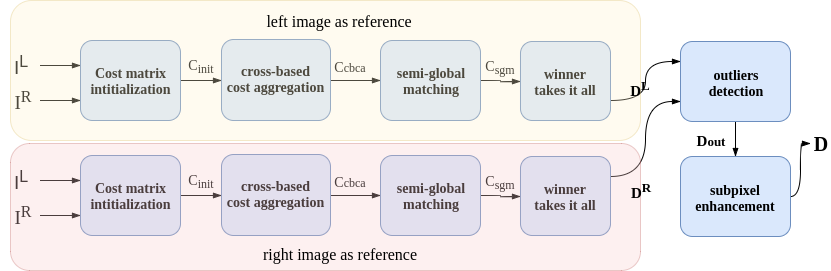
\includegraphics[scale=0.41]{method_diagram.png}
\end{frame}

%%%%%%%%%%%%%%%%%%%%%%%%%%%%% new frame %%%%%%%%%%%%%%%%%%%%%%%%%%%%%%%%%%%%%%%
\begin{frame}{Ενδεικτικό παράδειγμα ολόκληρης μεθόδου}
\begin{columns}[onlytextwidth]
\column{0.2\textwidth}
\begin{itemize}
	\item μέσο απόλυτο σφάλμα: $0.62 px$
	\item ποσοστό σφάλματος: $2.67\%$
	\item μέθοδος \e AD-Census: \g $5.422\%$
\end{itemize}
\column{0.8\textwidth}
\begin{figure}
	\centering
	\begin{subfigure}{\textwidth}
	\centering
	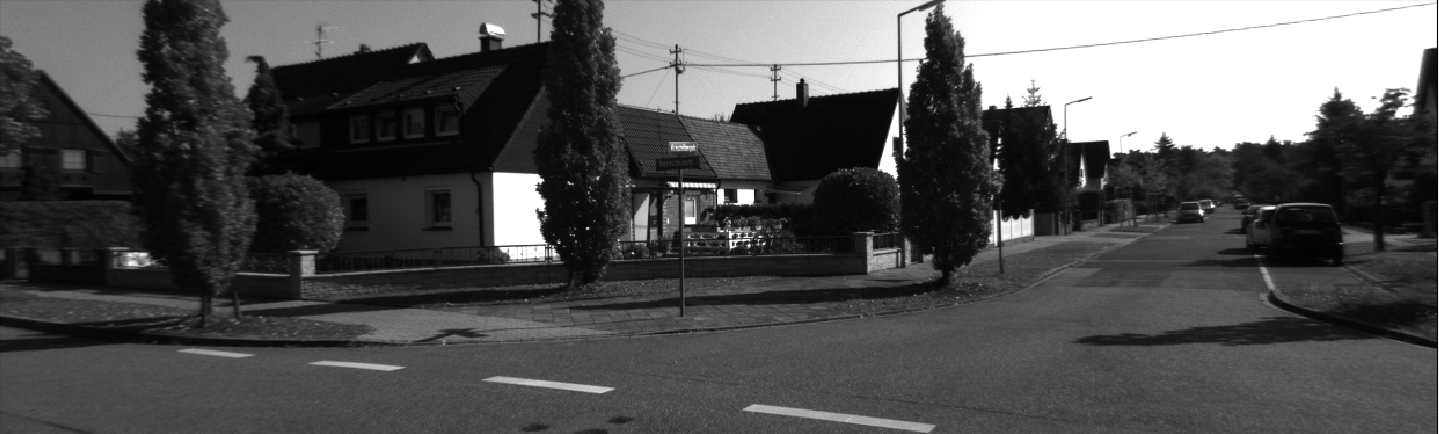
\includegraphics[height=20mm]{im4_imL.png}
	\end{subfigure}
	
	\begin{subfigure}{\textwidth}
	\centering
	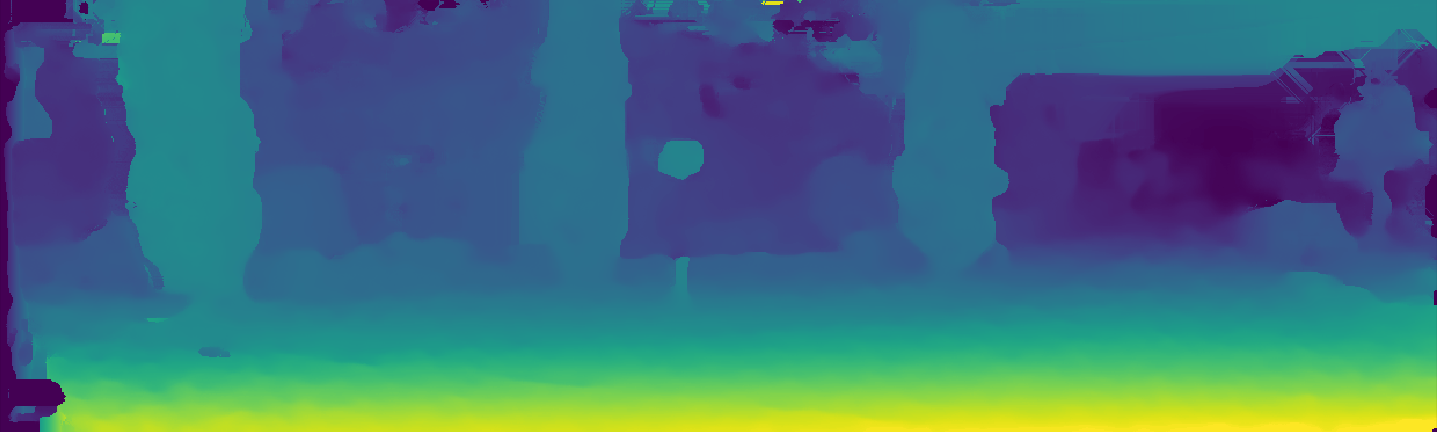
\includegraphics[height=20mm]{cnn_cbca30_sgm_outliers_subpixel.png}
	\end{subfigure}
	
	\begin{subfigure}{\textwidth}
	\centering
	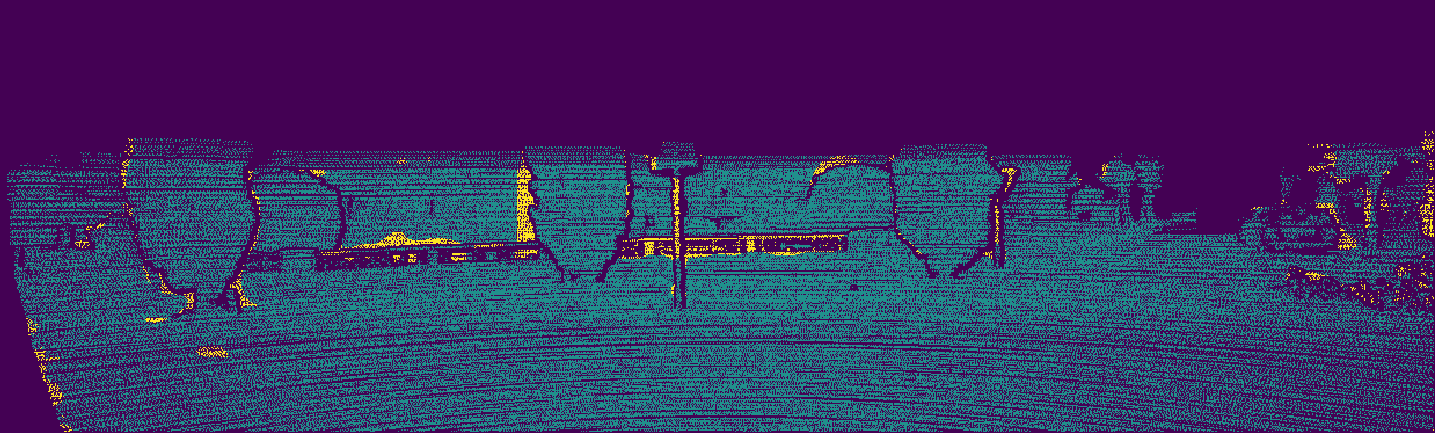
\includegraphics[height=20mm]{cnn_cbca30_sgm_outliers_subpixel_error_thres.png}
	\end{subfigure}
\end{figure}
\end{columns}
\end{frame}

%%%%%%%%%%%%%%%%%%%%%%%%%%%%% new frame %%%%%%%%%%%%%%%%%%%%%%%%%%%%%%%%%%%%%%%
\begin{frame}{Από τα καλύτερα}
\begin{columns}[onlytextwidth]
\column{0.2\textwidth}
\begin{itemize}
	\item μέσο απόλυτο σφάλμα: $1.577 px$
	\item ποσοστό σφάλματος: $1.248\%$
\end{itemize}
\column{0.8\textwidth}
\begin{figure}
	\centering
	\begin{subfigure}{\textwidth}
	\centering
	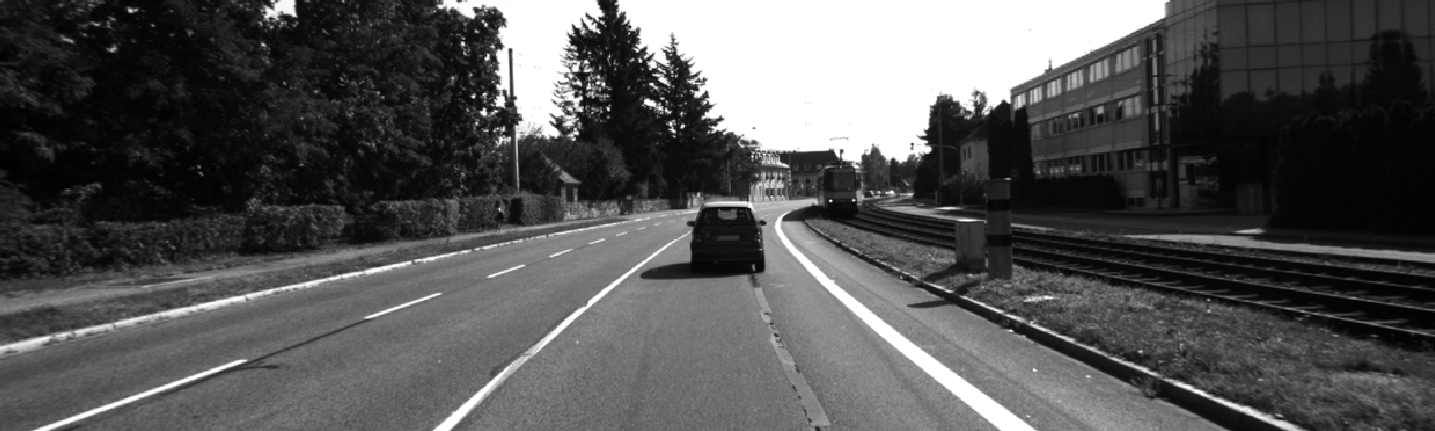
\includegraphics[height=20mm]{kitti2015_best_imL.png}
	\end{subfigure}
	
	\begin{subfigure}{\textwidth}
	\centering
	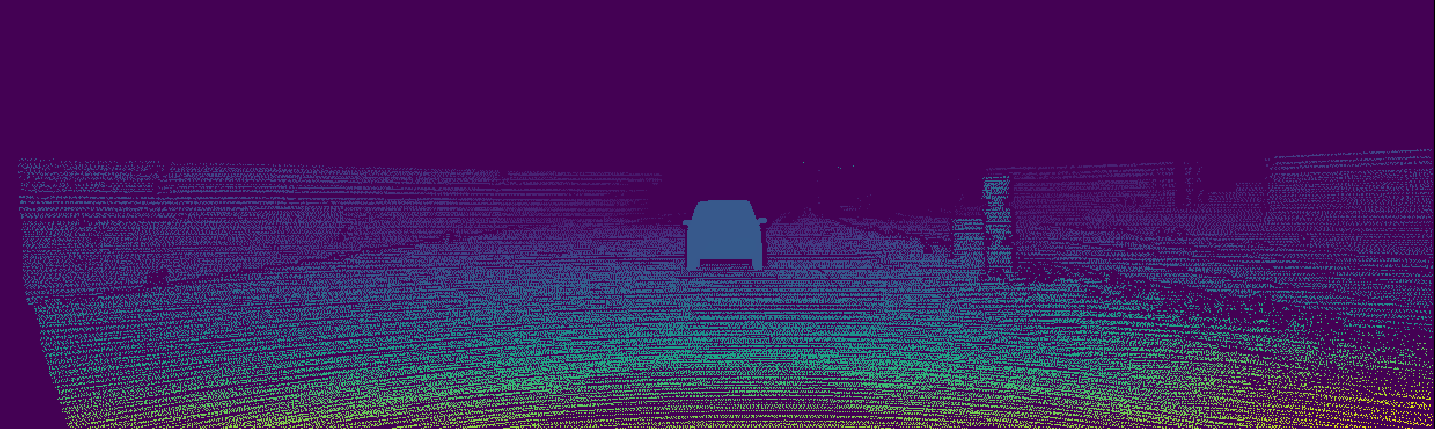
\includegraphics[height=20mm]{kitti2015_best_disparity_gt.png}
	\end{subfigure}
	
	\begin{subfigure}{\textwidth}
	\centering
	
\includegraphics[height=20mm]{kitti2015_best_disparity_pred.png}
	\end{subfigure}
\end{figure}
\end{columns}
\end{frame}

%%%%%%%%%%%%%%%%%%%%%%%%%%%%% new frame %%%%%%%%%%%%%%%%%%%%%%%%%%%%%%%%%%%%%%%
\begin{frame}{Από τα χειρότερα}
\begin{columns}[onlytextwidth]
\column{0.2\textwidth}
\begin{itemize}
	\item μέσο απόλυτο σφάλμα: $9.98 px$
	\item ποσοστό σφάλματος: $29.61\%$
\end{itemize}
\column{0.8\textwidth}
\begin{figure}
	\centering
	\begin{subfigure}{\textwidth}
	\centering
	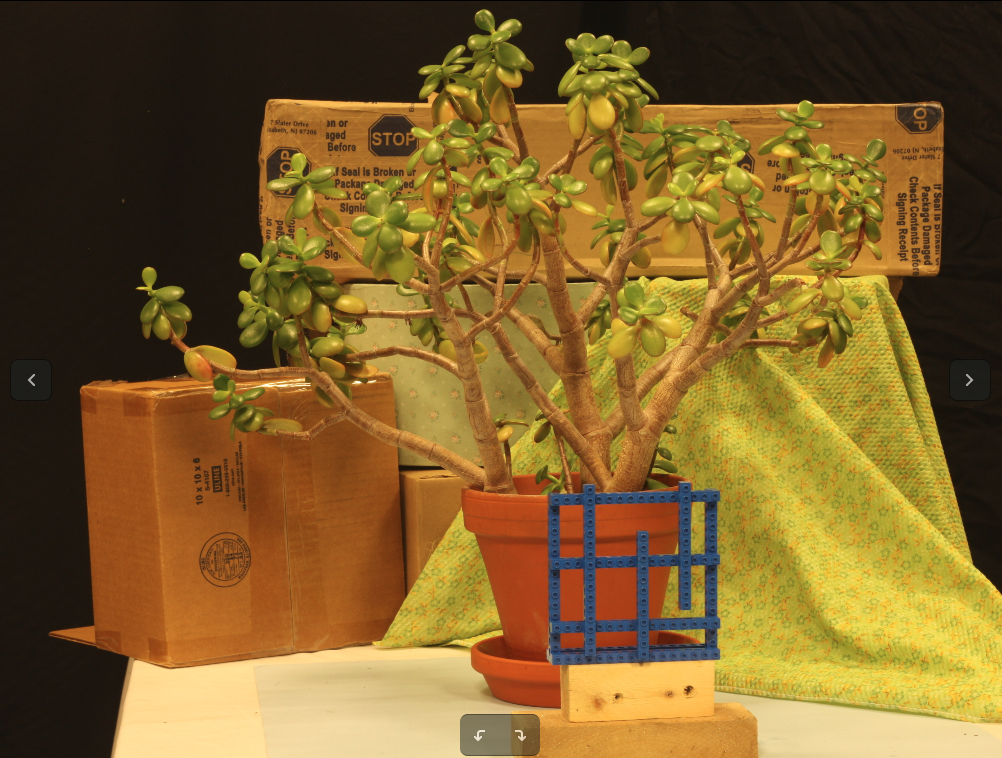
\includegraphics[height=30mm]{mb_worst_imL.png}
	\end{subfigure}
	
	\begin{subfigure}{\textwidth}
	\centering
	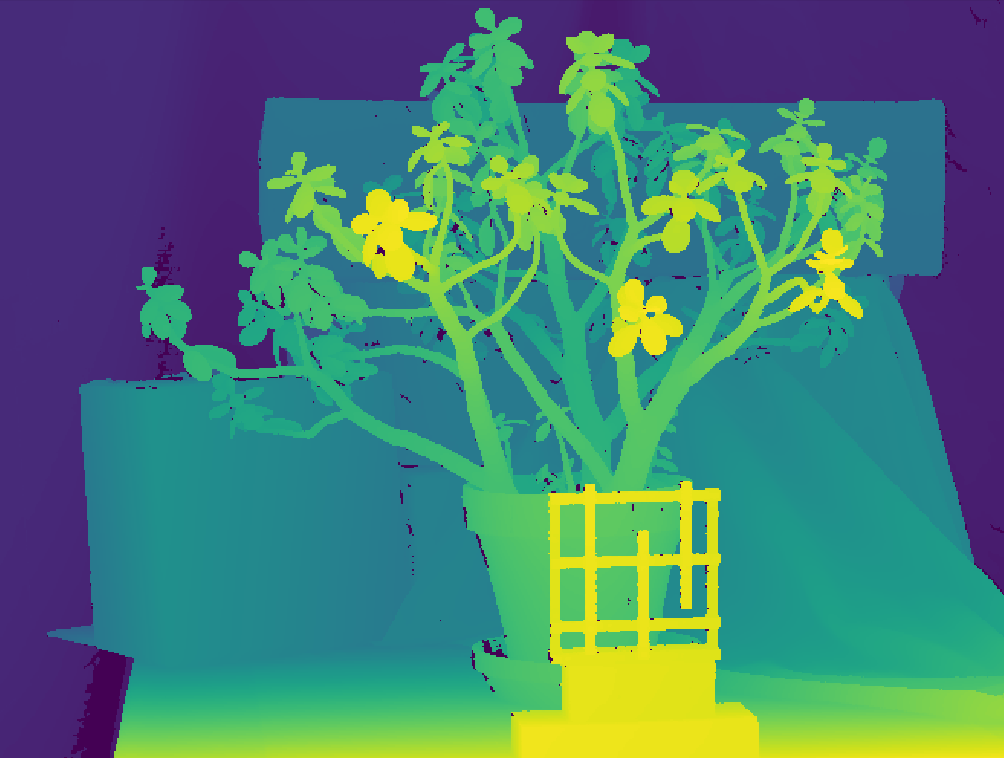
\includegraphics[height=30mm]{mb_worst_disparity_gt.png}
	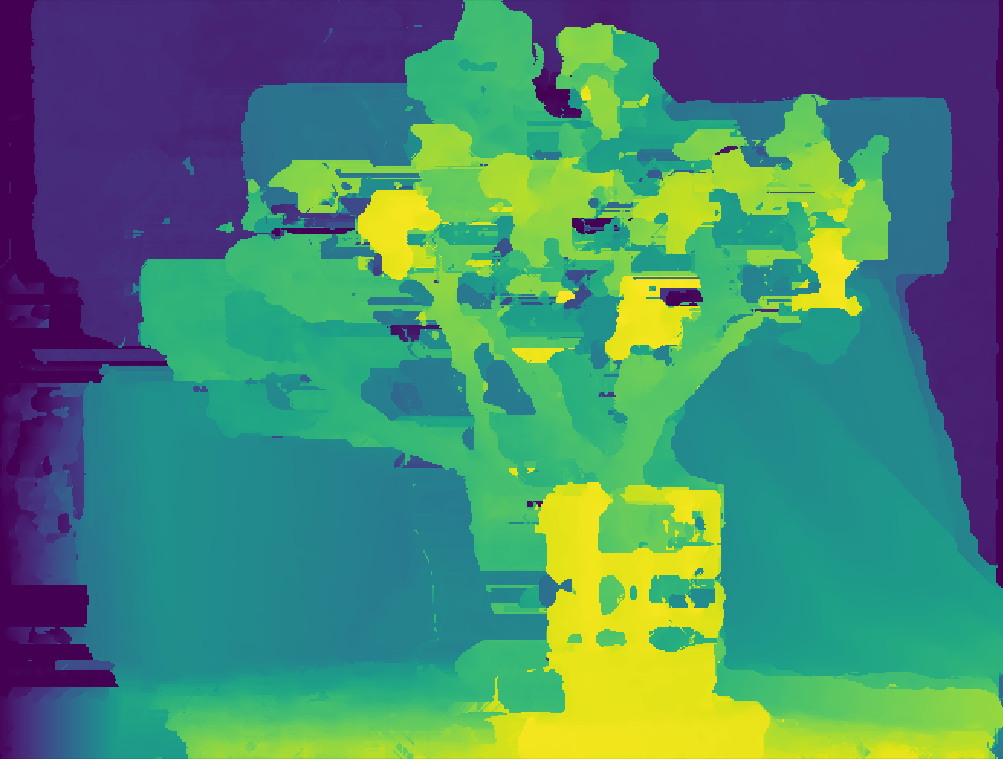
\includegraphics[height=30mm]{mb_worst_disparity_pred.png}
	\end{subfigure}
\end{figure}
\end{columns}
\end{frame}

%%%%%%%%%%%%%%%%%%%%%%%%%%%%% new frame %%%%%%%%%%%%%%%%%%%%%%%%%%%%%%%%%%%%%%%
\begin{frame}{Αποτελέσματα - ΚΙΤΤΙ 2012}
\centering
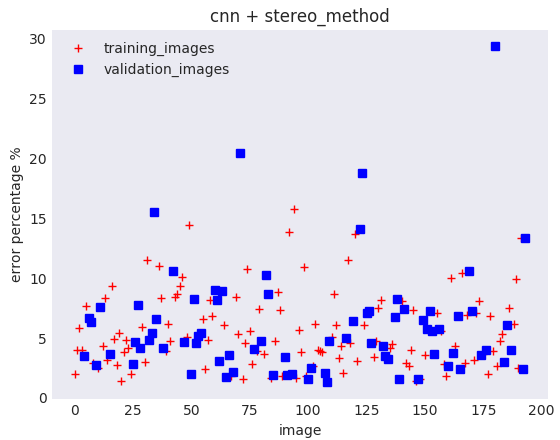
\includegraphics[scale=0.45]{kitti2012_cnn_stereo_method_error_per_image.png}
\end{frame}


%%%%%%%%%%%%%%%%%%%%%%%%%%%%% new frame %%%%%%%%%%%%%%%%%%%%%%%%%%%%%%%%%%%%%%%
\begin{frame}{Αποτελέσματα - Απόλυτο σφάλμα με ανώφλι}
\centering
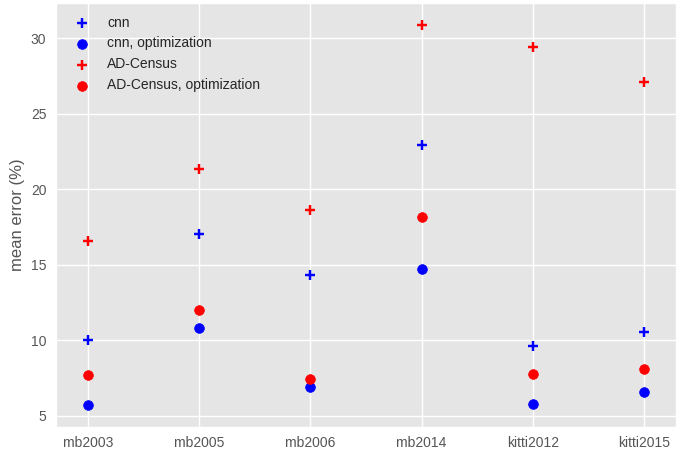
\includegraphics[scale=0.4]{absolute_error_thres.png}
\end{frame}

%%%%%%%%%%%%%%%%%%%%%%%%%%%%% new frame %%%%%%%%%%%%%%%%%%%%%%%%%%%%%%%%%%%%%%%
\begin{frame}{Αποτελέσματα - Απόλυτο σφάλμα}
\centering
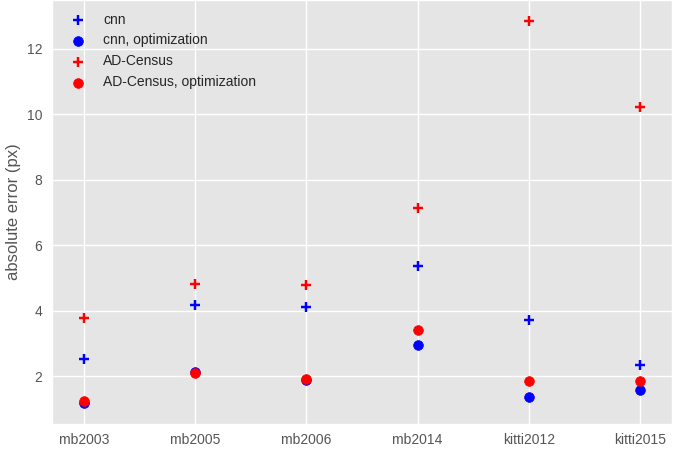
\includegraphics[scale=0.4]{absolute_error.png}
\end{frame}

%%%%%%%%%%%%%%%%%%%%%%%%%%%%% new frame %%%%%%%%%%%%%%%%%%%%%%%%%%%%%%%%%%%%%%%
\begin{frame}{Αποτελέσματα - Χρόνοι εκτέλεσης νευρωνικού}
\centering
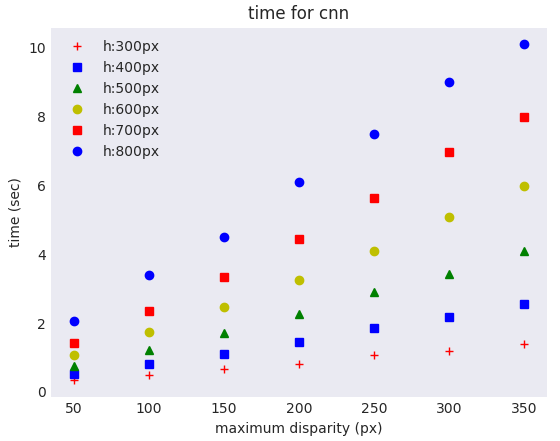
\includegraphics[scale=0.45]{cnn_times.png}
\end{frame}

%%%%%%%%%%%%%%%%%%%%%%%%%%%%% new frame %%%%%%%%%%%%%%%%%%%%%%%%%%%%%%%%%%%%%%%
\begin{frame}{Συμπεράσματα}
\fontsize{10}{7.2}\selectfont
\begin{itemize}
	\item \e Cnn \g βελτιώνουν εξαιρετικά την ακρίβεια της μεθοδολογίας
	\item Αρκετά καλή γενίκευση, ακόμα και σε στερεοσκοπικά ζεύγη τελείως διαφορετικής στατιστικής
\end{itemize}

Δυσκολίες:
\begin{itemize}
	\item Υπολογιστική πολυπλοκότητα - απαραίτητη \e GPU \g - αδύνατο να τρέξει απευθείας σε \e hardware \g κινητού, απαραίτητη μεσολάβηση \e server \g
	\item Χρόνοι $\approx 1 \sfrac{sec}{image}$ - χρειάζεται επιτάχυνση $25x$ για \e live video \g
\end{itemize}

Προτάσεις:
\begin{itemize}
	\item Μοντελοποίηση βημάτων 2, 3 με μηχανική μάθηση (δυσκολία στην πράξη $argmin$)
	\item Εξερεύνηση τεχνικών \e unsupervised learning \g (πχ μέσω \e reprojection error) \g
	\item Βάθος από μια λήψη
	\item Μείωση χρόνου εκτέλεσης
\end{itemize}
	
\end{frame}

\begin{frame}{Ενδεικτική Βιβλιογραφία}

\e
\begin{itemize}
	\item Jure Zbontar and Yann LeCun (2016): “Stereo matching by training a convolutional
neural network to compare image patches”
	\item Wenjie Luo, Alexander G. Schwing and Raquel Urtasun (2016): “Efficient Deep Learn-
ing for Stereo Matching”
	\item Xing Mei et al (2011): “On building an accurate stereo matching system on graphics
hardware”
	\item Heiko Hirschmuller (2008): “Stereo processing by semiglobal matching and mutual in-
formation”
\end{itemize}

	
\end{frame}

\begin{frame}{Τέλος}
\centering
Ευχαριστώ πολύ για την προσοχή σας!

Ερωτήσεις?

\begin{figure}
	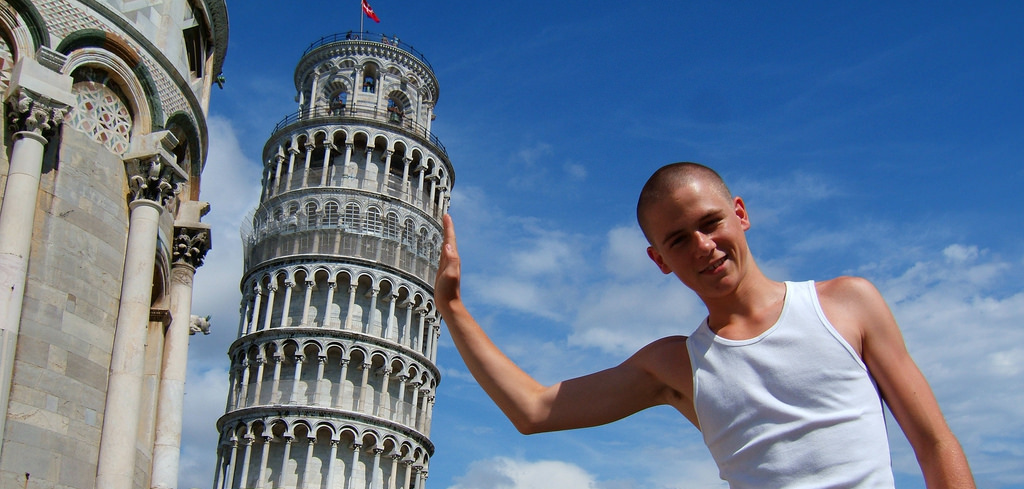
\includegraphics[scale=0.35]{illusion.png}
\end{figure}
	
\end{frame}

\end{document}
